\documentclass[12pt
,headinclude
,headsepline
,bibtotocnumbered
]{scrartcl}
\usepackage[paper=a4paper,left=25mm,right=25mm,top=25mm,bottom=25mm]{geometry} 
\usepackage[utf8]{inputenc}
\usepackage[english]{babel}
\usepackage{fancyvrb}  % Add this line
\usepackage{graphicx}
\usepackage{multirow}
\usepackage{pdfpages}
%\usepackage{wrapfig}
\usepackage{placeins}
\usepackage{float}
\usepackage{flafter}
\usepackage{mathtools}
\usepackage{hyperref}
\usepackage{epstopdf}
\usepackage[miktex]{gnuplottex}
\usepackage[T1]{fontenc}
\usepackage{mhchem}
\usepackage{fancyhdr}
%\setlength{\mathindent}{0pt}
\usepackage{amssymb}
\usepackage[list=true, font=large, labelfont=bf, 
labelformat=brace, position=top]{subcaption}
\setlength{\parindent}{0mm}
\usepackage{listings}
\usepackage{color}

\definecolor{dkgreen}{rgb}{0,0.6,0}
\definecolor{gray}{rgb}{0.5,0.5,0.5}
\definecolor{mauve}{rgb}{0.58,0,0.82}

\lstset{ %
	language=Python,                % the language of the code
	basicstyle=\small\ttfamily,     % the size of the fonts that are used for the code
	numbers=left,                   % where to put the line-numbers
	numberstyle=\tiny\color{gray},  % the style that is used for the line-numbers
	stepnumber=1,                   % the step between two line-numbers. If it's 1, each line will be numbered
	numbersep=5pt,                  % how far the line-numbers are from the code
	backgroundcolor=\color{white},  % choose the background color. You must add \usepackage{color}
	showspaces=false,               % show spaces adding particular underscores
	showstringspaces=false,         % underline spaces within strings
	showtabs=false,                 % show tabs within strings adding particular underscores
	frame=single,                   % adds a frame around the code
	rulecolor=\color{black},        % if not set, the frame-color may be changed on line-breaks within not-black text (e.g. commens (green here))
	tabsize=2,                      % sets default tabsize to 2 spaces
	captionpos=b,                   % sets the caption-position to bottom
	breaklines=true,                % sets automatic line breaking
	breakatwhitespace=true,         % sets if automatic breaks should only happen at whitespace
	title=\lstname,                 % show the filename of files included with \lstinputlisting; also try caption instead of title
	keywordstyle=\color{blue},      % keyword style
	commentstyle=\color{dkgreen},   % comment style
	stringstyle=\color{mauve},      % string literal style
	escapeinside={\%*}{*)},         % if you want to add LaTeX within your code
	morekeywords={*,...}            % if you want to add more keywords to the set
}

\setlength{\parindent}{0mm}

\pagestyle{fancy}
\fancyhf{}
\lhead{PRE-T\\ Exercise 4:Maximum-Likelihood - Bayesian Classification}
\rhead{Hsin-Feng Ho \\03770686}
\rfoot{Page \thepage}	
\begin{document}
\section*{Introduction}
In this exercise, we will use the maximum likelihood method to perform a Gaussian Naive Bayes classification. Two clips of Landsat satellite images with 7 different spectral channels are given. The first clip is used as training data and the second clip is used as test data. The goal is to classify the pixels of the test data into one of the 7 classes. The classes are: water, forest, vegetation, ice, snow, rock, shadow. 
\section*{Training data and test data}
Firstly we want to visualize the training data and the ground truth label of the training data.
\begin{figure}[H]
\centering
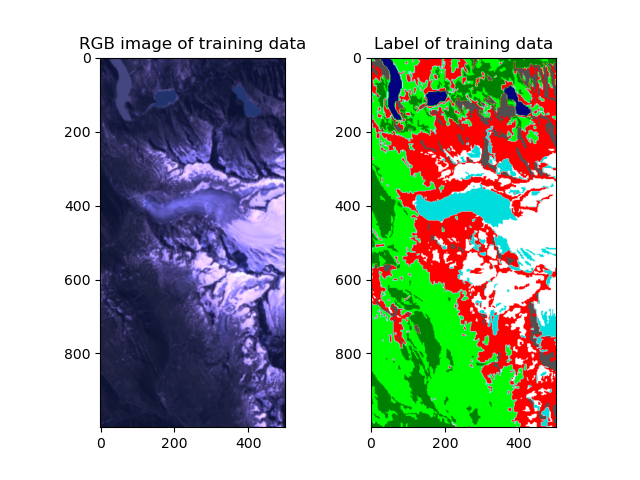
\includegraphics[width=1\textwidth]{plots/train.png}
\end{figure}
We can see that is hard to distinguish the classes by only looking at the spectral channels. However, we can see that the water and the shadow classes are quite different from the other classes. The water class has a very low reflectance in all spectral channels. The shadow class has a very low reflectance in the visible spectral channels. The other classes have similar reflectance in the visible spectral channels. However, they have different reflectance in the infrared spectral channels. Therefore, we can expect that the infrared spectral channels are more important for the classification.
\section*{Maximum likelihood method}
The maximum likelihood method is a method to estimate the parameters of a probability distribution. The probability distribution is assumed to be a Gaussian distribution. The probability density function of a Gaussian distribution is
\begin{equation*}
    p(\boldsymbol{x}|\omega_i)=\frac{1}{(2\pi)^{\frac{N}{2}}\sqrt{|\boldsymbol{K_{xxi}}|}}\exp{\left\{-\frac{1}{2}(\boldsymbol{x}-\boldsymbol{m_i})^T\boldsymbol{K_{xxi}}^{-1}(\boldsymbol{x}-\boldsymbol{m_i})\right\}}
\end{equation*}
where $\boldsymbol{x}$ is a vector of the spectral channels, $\omega_i$ is the class, $N$ is the number of spectral channels, $\boldsymbol{m_i}$ is the mean vector of the class $\omega_i$ and $\boldsymbol{K_{xxi}}$ is the covariance matrix of the class $\omega_i$.
\subsection*{Training the classifier}
Now we have to train our classifier with the training data. We use the maximum likelihood method to estimate the parameters of the Gaussian Naive Bayes classifier.
\begin{lstlisting}[breaklines=true]
    clf=GaussianNB()
    clf.fit(X_train,y_train)
    y_pred=clf.predict(X_train)
\end{lstlisting}
Now we want to visualize the classification result of the training data.
\begin{figure}[H]
\centering
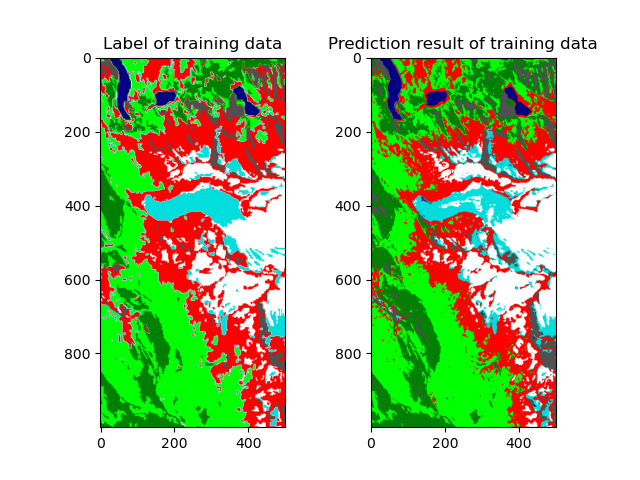
\includegraphics[width=1\textwidth]{plots/train_result.png}
\end{figure}
We can see that the water and rock classes are classified very well. However, the other classes for example vegetation and forest, ice and snow are not classified very well. The reason is that the other classes have similar reflectance in the spectral channels. Therefore, it is hard to distinguish them.
\subsection*{Prediction on the test data}
Now we want to visualize the test data and the ground truth label of the test data.
\begin{figure}[H]
\centering
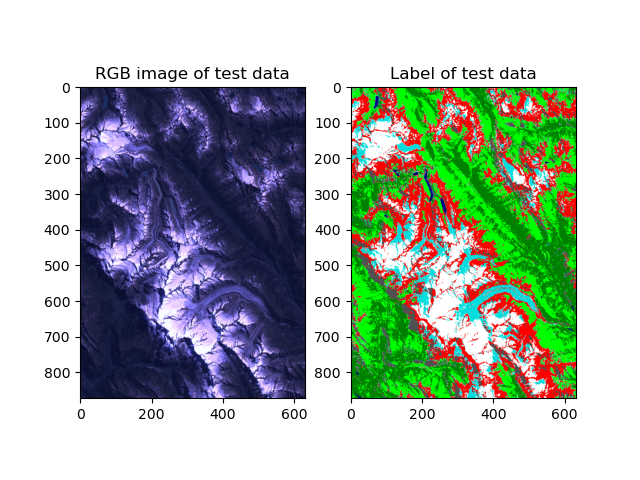
\includegraphics[width=1\textwidth]{plots/test.png}
\end{figure}
We can predict the classes of the test data with our trained classifier.
\begin{lstlisting}[breaklines=true]
    y_pred=clf.predict(X_test)
\end{lstlisting}
Now we want to visualize the classification result of the test data.
\begin{figure}[H]
\centering
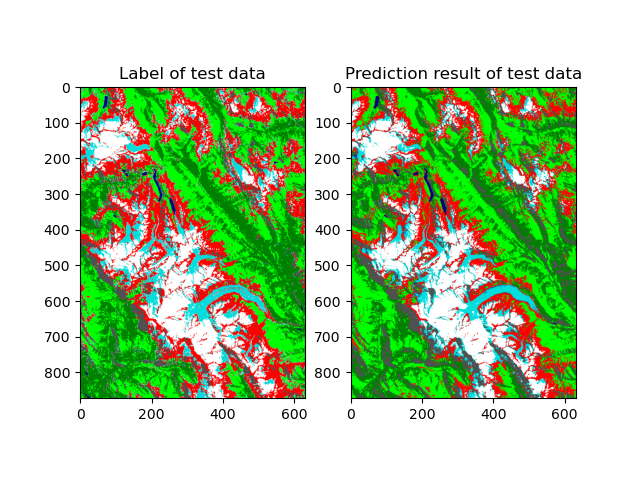
\includegraphics[width=1\textwidth]{plots/test_result.png}
\end{figure}
The same as the training data, the classifation of the water and rocks are better than other classes. In the test data, the snow and ice are slightly better classified than in the train image. However, the vegetation and forest are still not classified very well. 
\subsection*{Confusion matrix}
We can also observe the confusion matrix of the classification result. The confusion matrix is a matrix which shows the number of samples of the true class and the predicted class. The diagonal elements of the confusion matrix are the number of samples which are correctly classified. The off-diagonal elements of the confusion matrix are the number of samples which are incorrectly classified.
\\\\
There are several accuracies which can be calculated from the confusion matrix. The user's accuracy is the number of correctly classified samples divided by the number of samples which are predicted to be in the class. The producer's accuracy is the number of correctly classified samples divided by the number of samples which are actually in the class. The overall accuracy is the number of correctly classified samples divided by the total number of samples.
\begin{table}[H]
    \renewcommand\arraystretch{1.5}
    \setlength{\tabcolsep}{0.7mm}{
    \begin{tabular}{|c|c|c|c|c|c|c|c|c|c|c|}
        \hline
        \multicolumn{2}{|c|}{\multirow{2}{*}{Class}}&\multicolumn{7}{c}{Reference data}&&Accuracy\\\cline{3-11}
        \multicolumn{2}{|c|}{}&Water&Forest&Vegetation&Ice&Snow&Rock&Shadow&Total&User's\\
    \hline
    \multirow{7}{*}{Predict}&Water&\textbf{1481}&39&12&619&189&94&91&2525&0.586\\
    \cline{2-11}
    &Forest&34&\textbf{81218}&11094&2083&1074&7305&1832&104640&0.776\\
    \cline{2-11}
    &Vegetation&0&17381&\textbf{112113}&5362&2123&13203&288&150470&0.745\\
    \cline{2-11}
    &Ice&3&20&23&\textbf{29524}&7611&6353&369&43903&0.672\\
    \cline{2-11}
    &Snow&0&0&0&8515&\textbf{70736}&2507&0&81758&0.865\\
    \cline{2-11}
    &Rock&6&94&5717&4447&5252&\textbf{86618}&12710&102495&0.845\\
    \cline{2-11}
    &Shadow&401&14564&457&2253&1575&12710&\textbf{33353}&65313&0.511\\\cline{2-11}
    &Total&1925&113316&129416&52803&88560&128790&36294&\textbf{551104}&\\\hline
    Accuracy&Producer's&0.769&0.717&0.866&0.559&0.799&0.672&0.919&&\textbf{0.769}\\
    \hline
    \end{tabular}}
\end{table}
From the user's accuracy, we can see that the snow and rock classes are classified very well. The forest, vegetation, ice classes are classified quite well. The accuracies of water and shadow are just over 50\%. We achieve an overall accuracy of 76.9\%. 
\subsection*{Kappa coefficient}
The kappa coefficient is a measure of the agreement between the predicted class and the true class. The kappa coefficient is defined as
\begin{equation*}
    \kappa=\frac{p_o-p_e}{1-p_e}=\frac{n\sum_{i=1}^{m}n_{ii}-\sum_{i=1}^{m}n_{i+}n_{+i}}{n^2-\sum_{i=1}^{m}n_{i+}n_{+i}}
\end{equation*}
where $p_o$ is the observed agreement, $p_e$ is the expected agreement, $n$ is the total number of samples, $n_{ii}$ is the number of samples which are correctly classified, $n_{i+}$ is the number of samples which are predicted to be in the class $i$, $n_{+i}$ is the number of samples which are actually in the class $i$ and $m$ is the number of classes.
\begin{verbatim}
    Kappa coefficient:  0.6967297666414108
\end{verbatim}
The result of kappa coefficient is 0.6967. The kappa coefficient is between 0 and 1. The kappa coefficient is 1 if the predicted class is the same as the true class. The kappa coefficient is 0 if the predicted class is the same as the true class by chance. The kappa coefficient is negative if the predicted class is worse than the true class. Therefore, we can say that our classifier is much better than random guessing.
\section*{Train only on RGB channels}
Now we want to train our classifier only on the RGB channels. We want to see if the infrared channels are important for the classification.
\begin{figure}[H]
\centering
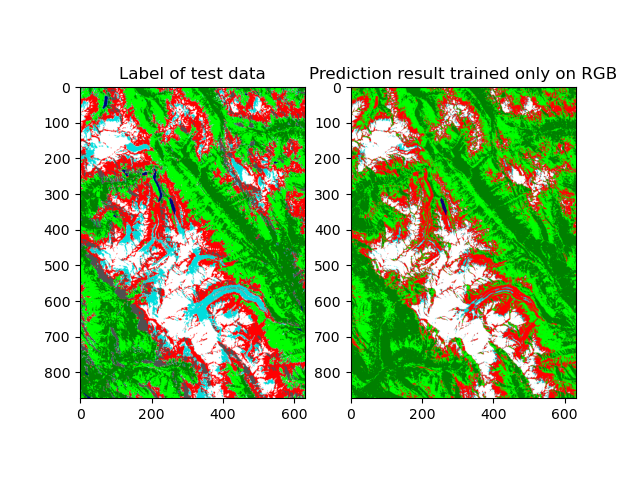
\includegraphics[width=1\textwidth]{plots/test_result_rgb.png}
\end{figure}
\begin{table}[H]
    \renewcommand\arraystretch{1.5}
    \setlength{\tabcolsep}{0.7mm}{
    \begin{tabular}{|c|c|c|c|c|c|c|c|c|c|c|}
        \hline
        \multicolumn{2}{|c|}{\multirow{2}{*}{Class}}&\multicolumn{7}{c}{Reference data}&&Accuracy\\\cline{3-11}
        \multicolumn{2}{|c|}{}&Water&Forest&Vegetation&Ice&Snow&Rock&Shadow&Total&User's\\
    \hline
    \multirow{7}{*}{Predict}&Water&\textbf{349}&345&112&0&0&1119&0&1925&0.181\\
    \cline{2-11}
    &Forest&6&\textbf{100562}&12576&0&0&172&0&113316&0.887\\
    \cline{2-11}
    &Vegetation&9&29693&\textbf{92876}&0&0&6838&0&129416&0.718\\
    \cline{2-11}
    &Ice&5&2771&7041&\textbf{9826}&9467&23693&0&52803&0.186\\
    \cline{2-11}
    &Snow&2&1338&3815&2868&\textbf{70922}&9615&0&88560&0.801\\
    \cline{2-11}
    &Rock&1&6854&33914&5716&4546&\textbf{77753}&6&128790&0.604\\
    \cline{2-11}
    &Shadow&0&30079&5670&0&0&524&\textbf{21}&36294&5.786$\cdot 10^{-4}$\\\cline{2-11}
    &Total&372&171642&156004 &18410 &84935&119714& 27&\textbf{551104}&\\\hline
    Accuracy&Producer's&0.938&0.586&0.595&0.534&0.835&0.650&0.778&&\textbf{0.639}\\
    \hline
    \end{tabular}}
\end{table}
\end{document}
